\documentclass{beamer}

\setbeamertemplate{bibliography entry title}{}
\setbeamertemplate{bibliography entry location}{}
\setbeamertemplate{bibliography entry note}{}

\usepackage{amsmath}
% TikZ
\usepackage{tikz}
\tikzset{
  level/.style={
    sibling distance=40mm/#1
  },
  level distance=10mm,
}

 \tikzset{
  every node/.style={
    draw,
    circle,
    inner sep=0pt,
    minimum width=15pt
  },
  thick
}
% Code representation, thanks to github:anaechavarria for this config.
\usepackage{listings}
\renewcommand{\lstlistingname}{Código}
\lstset{
	language=Python,               % Lenguaje
	basicstyle=\ttfamily\footnotesize,  % Tipo de fuente
	keywordstyle=\color{blue},  % Color de palabras clave
	stringstyle=\color{red},    % Color de strings
	commentstyle=\color{gray},  % Color de comentarios
	showstringspaces=false,     % No muestrar el _ cuando el string tiene espacios
	breaklines = true,          % Partir las líneas largas
	breakatwhitespace=true,	    % Partir las líneas en un espacio
	% numbers=left,				% Numerar las líneas a la izq
	numberstyle=\tiny,			% Poner los números de las líneas pequeños
	numberblanklines=false,      % Numerar las líneas en blanco
	columns=fullflexible,       % No perder el formato al dejar los espacios
	keepspaces=true,   			% Dejar los espacios insertados
	frame=tb,					% Poner el recuadro
}




\title[]{Proseminar Theoretische Informatik}
\subtitle{Dynamic Programming}
\author{Juan Andrés Osorio Escobar}
\date{\today}
\usetheme{Madrid}

\begin{document}
  \input{presentation/slide_title}
  \input{presentation/slide_contents}
  \section{Introduction}
\subsection{Definition}

\begin{frame}
  \frametitle{Introduction}
  \begin{block}{Definition}
   What is Dynamic Programming?
   \begin{itemize}
     \item Problem Solving Paradigm
     \item Algorithm Design Technique
   \end{itemize}
  \end{block}
\end{frame}

\begin{frame}
  \frametitle{Introduction}
  \begin{block}{Key Properties}
   A problem which is solvable through Dynamic
   Programming has the following properties:
   \begin{itemize}
     \item Optimal Substructure
     \item Overlapping Subproblems
   \end{itemize}
  \end{block}

  % \begin{alertblock}{}
  %   here is some thext
  % \end{alertblock}
\end{frame}

\subsection{Fibonacci Sequence}
\begin{frame}
  \frametitle{Introduction - Fibonacci Sequence}
  Let us first take a look at a simple Dynamic Programming approach.

  \begin{block}{Example}
    The Fibonacci sequence is defined as follows:
    \\
    \[
    fib(n) = \left\{\begin{array}{lr}
      1, & \text{for } n = 0, n = 1\\
      fib(n-1) + fib(n-2), & \text{otherwise}
      \end{array}\right\}
    \]
    \\
  \end{block}
\end{frame}



\begin{frame}[fragile]
  \frametitle{Introduction - Fibonacci Sequence}
  \begin{block}{Example}
    A naive solution for computing the n-th number in the 
    Fibonacci sequence:
  \end{block}
  \begin{lstlisting}

      def fibonacci(n):
        if (n <= 1):
          return 1
        else:
          return fibonacci(n - 1) + fibonacci(n - 2)

    \end{lstlisting}
\end{frame}


\begin{frame}
\frametitle{Introduction - Fibonacci Sequence}
\begin{figure}[ht]
  \centering
  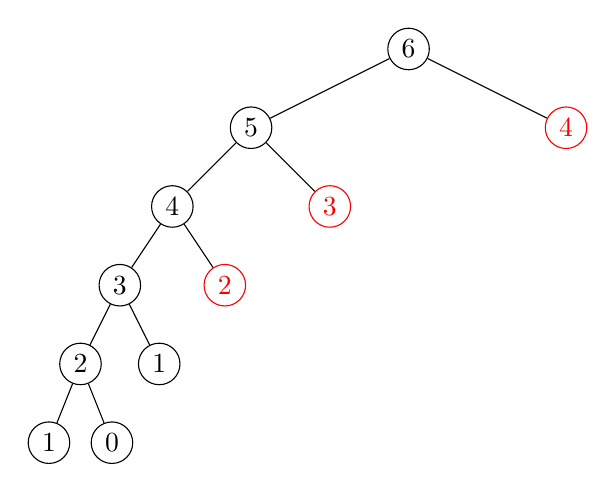
\begin{tikzpicture}
    \node {6}
      child { node {5}
        child { node {4} 
          child{ node {3} 
            child { node {2}
              child {node {1}}
              child {node {0}}
            }
            child { node {1}}
          }
          child{ node[color=red] {2} }
        }
        child { node[color=red] {3} }
      }
      child { node[color=red] {4}
      };
  \end{tikzpicture}
  \caption{Fibonacci recursion tree with $n = 6$}
\end{figure}
\end{frame}

\begin{frame}
% \frametitle{Introduction - Fibonacci Sequence}
\begin{figure}[ht]
  \centering
  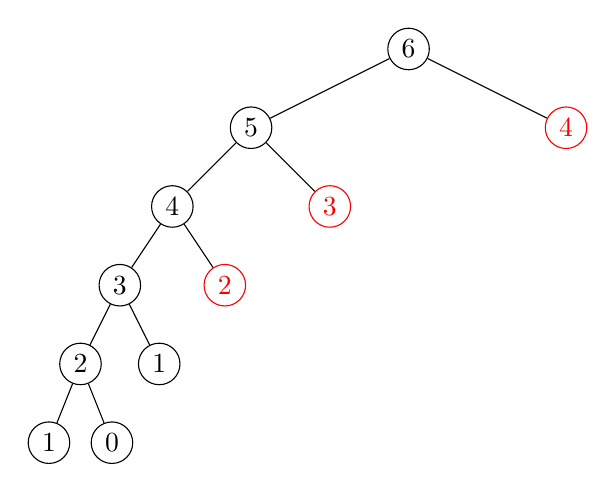
\begin{tikzpicture}
    \node {6}
      child { node {5}
        child { node {4} 
          child{ node {3} 
            child { node {2}
              child {node {1}}
              child {node {0}}
            }
            child { node {1}}
          }
          child{ node[color=red] {2} }
        }
        child { node[color=red] {3} }
      }
      child { node[color=red] {4}
      };
  \end{tikzpicture}
  \caption{Fibonacci recursion tree with $n = 6$}
\end{figure}
\begin{alertblock}{!}
  Every red-colored Node is a computation we are doing not for the
  first time!
\end{alertblock}
\end{frame}


\begin{frame}[fragile]
  \frametitle{Introduction - Fibonacci Sequence}
  \begin{block}{Dynamic Programming Approach}
    How about we keep record of the values we compute?
  \end{block}
  \begin{lstlisting}
    # initialize the look up table with 
    # non-recursively defined fibonacci numbers.
    look_up_table = {
      0: 1,
      1: 1  
    }

    def dp_fibonacci(n):
      if (look_up_table.at(n)):
        return look_up_table.at(n)
      else :
        look_up_table[n] = dp_fibonacci(n - 1) + dp_fibonacci(n - 2)
        return look_up_table[n]
  \end{lstlisting}
\end{frame}


\begin{frame}
  \begin{block}{Discussion}
    Our modifications to the original approach have
    caused changes in the following aspects in our program:
    \begin{itemize}
      \item Memory Usage
      \item Time needed to compute the solution
    \end{itemize}
  \end{block}
\end{frame}
  \section{Elements Of Dynamic Programming}

% \begin{frame}{Elements Of Dynamic Programming}
%   \begin{block}{Key Aspects}
%     \begin{enumerate}
%       \item Optimal Substructures
%     \end{enumerate}
%   \end{block}
% \end{frame}


\begin{frame}{Elements Of Dynamic Programming}
  \begin{block}{Key Aspects}
    \begin{enumerate}
      \item Optimal Substructures
    \end{enumerate}
    \pause
    The solution for a subproblem is part of the solution of the original problem
  \end{block}
\end{frame}

% \begin{frame}{Elements Of Dynamic Programming}
%   \begin{block}{Key Aspects}
%     \begin{enumerate}
%       \item Optimal Substructres
%       \item Overlapping Subproblems
%     \end{enumerate}
%   \end{block}
% \end{frame}


\begin{frame}{Elements Of Dynamic Programming}
  \begin{block}{Key Aspects}
    \begin{enumerate}
      \item Optimal Substructures
      \item Overlapping Subproblems
    \end{enumerate}
    \pause
    When a recursive algorithm repeatedly revisits the same subproblem in different branches along its recursion
    tree, we say that the problem has overlapping subproblems.
  \end{block}
\end{frame}


\begin{frame}{Elements of DP: Rod-cutting Problem Example}
  Let us examine this properties based on the following problem:
  \begin{block}{Rod-cutting Problem Abridged Problem Statement}
  Given a rod of length n, and a table of prices $p_i$ for $i = 1, 2, ..., n$,
determine the maximum revenue $r_n$ obtained by cutting the rod and selling the pieces
  \end{block}
  %format differently?
\end{frame}

\begin{frame}{Elements of DP: Rod-cutting Problem Example}
  With the following Price Table:
  \\
  \vspace{2em}
\begin{table}[ht]
  \centering
  \begin{tabular}{l|ll}
    \textbf{length i}&\textbf{price $p_i$}\\\hline
      1 & 2\\
      2 & 6\\
      3 & 7\\
      4 & 8\\
      5 & 9
  \end{tabular}
\end{table}
\end{frame}
  \section{Matrix-chain Multiplication Problem}


\begin{frame}{Matrix-chain Multiplication Problem}
  It is known that multiplying matrices is a very frequent mathematical
  operation among the most varied application fields. Multiplying Matrices 
  $A_1$ and $A_2$ requires matching dimensions: the number of rows in $A_1$
  must match the number of columns in $A_2$ if one is to multiply the Matrices 
  in this order $A_{1}A_{2}$.
  \\
  \vspace{2em}
  The product obtained by multiplying a chain of matrices $A_{1}A_{2}...A_{n}$ 
  can be obtained by parenthesizing the chain in many different ways.
\end{frame}


\begin{frame}{Matrix-chain Multiplication Problem - Parenthesization}
  \begin{block}{Fully Parenthesized Product}
    A product of matrices is called \textbf{\emph{fully parenthesized}}
    either if it is a single matrix, or a fully parenthesized product of two matrixes, 
    surrounded by parenthesis.
  \end{block}
  \pause
  For example, a matrix chain consisting of the matrices $A_{1}A_{2}A_{3}A_{4}$ can be
  parenthesized in the following ways:
  \begin{itemize}
    \item $(((A_{1}A_{2})A_{3})A_{4})$
    \item $(A_{1}((A_{2}A_{3})A_{4}))$
    \item $(A_{1}(A_{2}(A_{3}A_{4})))$
    \item $((A_{1}(A_{2}A_{3}))A_{4})$
    \item $((A_{1}A_{2})(A_{3}A_{4}))$
  \end{itemize}
\end{frame}

\begin{frame}[allowframebreaks]{Matrix Multiplication Problem - Problem Statement}
  The way we parenthesize a matrix can have an enormous impact in the number
  of multiplications we have to compute in the end. 
  
  Take for example matrices $A_1$, $A_2$ and $A_3$ with dimensions $3 \times 50$, $50 \times 2$
  and $2 \times 40$ respectively, forming the chain $A_{1}A_{2}A_{3}$. we have the following parenthesization choices
  \\
  \vspace{0.5em}
  \begin{itemize}
    \item $((A_{1}A_{2})A_{3})$ yielding $3 \times 50 \times 2 + 3 \times 2 \times 40 = 540$ multiplications.
    \item  $(A_{1}(A_{2}A_{3}))$ yielding $50 \times 2 \times 40 + 3 \times 50 \times 40 = 10000$ multiplications.
  \end{itemize}

  \framebreak

  \begin{block}{Abridged Problem Statement}
    Given a chain of matrices $A_{1}A_{2}...A_{n}$, fully parenthesize the chain in a way
    that minimizes the amount of multiplications to be computed.
  \end{block}
\end{frame}

\begin{frame}[allowframebreaks]{Matrix-chain Multiplication Problem - Naive approach}
  Trying to solve this problem with a complete search approach leads us to the question:
  \\
  \vspace{1em}
  In how many different ways can we parenthesize a chain of n matrices?

  \framebreak
  when $n = 1$, the chain consists of only one matrix which we can only parenthesize in one way.
  when $n \geq 2$ a fully parenthesized matrix chain is the product of to fully parenthesized
  subproducts, and the split between two products may occur between the $kth$
  and the $(k + 1)st$ matrices for any $k = 1, 2, ..., n - 1 $. obtaining:
    \[
      P(n) = \left\{\begin{array}{lr}
        1, & \text{if } n = 1,\\
        \sum_{k=1}^{n-1}P(k)P(n-k), & \text{if } n \geq 2.
        \end{array}\right\}
    \]
  
  The time complexity for this recurrence is exponential! ($O(2^n)$)
\end{frame}

\begin{frame}{Matrix Multiplication Problem - Optimal Solution Structure}
  \begin{block}{Definition}
   Denote the matrix $A_{i...j}$ as the matrix obtained from the product
   of multiplying matrices $A_{i}A_{i+1}...A_{j}$ \\
  \vspace{0.5em}
  For the non trivial problem, we must split the product between matrices $A_k$ and $A_{k+1}$,
  with $ i \leq k < j$. The cost of parenthesizing this way is the cost
  of computing the matrix $A_{i...k}$, the cost of computing $A_{k+1...j}$,
  and the cost of multiplying both matrices together
  \end{block}

  \pause
  \begin{alertblock}{Optimality}
    An optimal parenthesization is composed of two optimal parenthesized matrix products as well,
    if any of these two composing it are not optimal parenthesizations, our optimal parenthesization can not be optimal,
    a contradiction!
  \end{alertblock}
\end{frame}

\begin{frame}{Matrix Multiplication Problem - Recursive Solution}
  % was meinte Clemens hier diesbezüglich? diese Formel verständlich
  % machen
    \[
    m[i,j] = \left\{\begin{array}{lr}
      0, & \text{if } i = j,\\
      min_{i \leq k < j} \{m[i,k] + m[k + 1, j] + p_{i-1}p_{k}p_{j}\} & \text{otherwise}
      \end{array}\right\}
    \]
  
\end{frame}

\begin{frame}{Matrix Multiplication Problem - Computing Optimal Costs}
  
\end{frame}

\begin{frame}{Matrix Multiplication Problem - Constructing an Optimal Solution}
  
\end{frame}
  \section{Top-down vs Bottom-up Approaches}


% nochmal tabular umgebung um diesen Fehler zu beheben.
\begin{frame}{Top-down vs Bottom-up Approaches}
  \begin{tabular}{ r | p{5cm} | p{5cm}}
   & \textbf{Top-Down} & \textbf{Bottom-Up} \\
   \hline
   Pros & Natural transformation from the complete search recursion & No overhead from recursive calls, faster in some scenarios \\
        & Computes the subproblems only when necessary & \\
   \hline
   Cons & Slower if many sub-problems are revisited due to function call overhead & For programmers who are inclined to recursion, this style may not be intuitive \\
        &                                                                         & Visits all the problem's states \\
  \end{tabular}
  \\
  \vspace{2em}
  \cite{halim2013competitive}
\end{frame}



  \begin{frame}[allowframebreaks]
        \frametitle{References}
        \bibliographystyle{amsalpha}
        \bibliography{./references.bib}
\end{frame}



\begin{frame}
  Thank you for your attention
  \\
  \vspace{5em}
  Questions?  
\end{frame}
\end{document}